\chapter{Immersed Boundary Methods}
\label{CHAPTER:IBM}.

\section{Overview of Immersed Boundary Methods}

\begin{figure}[!bp]
  \centering
  \subfloat[cartesian grid]{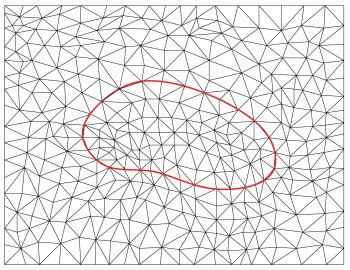
\includegraphics[width=0.4\textwidth]{gfx/immersed_boundary/general_partition_triangle.jpg}\label{fig:grid_f0}}
  \hfil
  \subfloat[unstructured body-fitted grid]{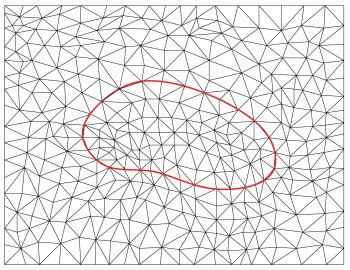
\includegraphics[width=0.4\textwidth]{gfx/immersed_boundary/general_partition_triangle.jpg}\label{fig:grid_f2}}
  \caption{Different types of numerical grids}
\end{figure}

For many fluid problems it is mandatory to solve the equations of motion with respect to complex-shaped geometries \.
The algorithm introduced in chapter \ref{CHAPTER:CUDA} is not yet suitable for such a scenario.
For instance the simulation inside a spheric geometry is impossible, since the boundaries
do not coincide with the implemented cartesian grid. Nevertheless there exist different approaches to overcome this problem,
which shall be introduced here. \\
The common approach to extend the algorithm would be to use a body-fitted mesh (see figure \ref{fig:grid_f1}),
different advantages and disadvantages arise with this kind of implementation (see \citep{Mittal2005}).
One benefit is a much simpler deployment of the desired boundary condition, due to the overlap of the grid with domain border.
Furthermore a higher accuracy can be achieved \citep{Gornak2013}.
However, using an unstructered grid generates plenty of computational overhead, during and before the execution of a simulation.
The generation of the grid is very complicated in contrast to using a cartesian grid, this can be even more complicated when
considering moving boundaries.
Also solving the finite differenc schemes on a curvilinear coordinate system, leads to more calculations on a single grid point.
The last important aspect is the implementation on the gpu.
Like discussed in section () it is more efficient to use homogenous storage and calculation pattern on a CUDA-device,
the use of unstructured data makes this very difficult.
Altough some attempts exists to solve these difficulties (see i.e. PAP), it is still uncertain if the obtained performance loss would be acceptable.\\
A set of alternative methods, to resolve the problems described above, are so called Immersed Boundary Methods.
The term was first mentioned in (PESKIN 1972), for the simulation of blood flow through a heartvale, but has since then been used for a variety of
methods (MITTAL).  All of them have the idea in common to perform the simulations on a cartesian grid which does not conform to the domain boundary.
To satisfy the desired boundary conditions additional terms are introduced into the equations of motion.
In general one can distinguish between contiuous forcing methods and direct forcing methods.
Continious forcing methods try to mimic the boundary using a localized force which acts on the boundary,
since the surface is tracked by lagrangian points this methods can be well suited for moving boundaries (MITTAL).
One common problem is that continous forcing can arise to stability problem and numerical oscillations in numericial stiff problem (SOURCE).
The direct forcing approach tries to satisfies the boundary condition, by imposing it directly to points near the fluid surface for example
trough an interpolaltion procedure.
Some of the major drawbacks using the IBM is the loss in  spatial accuracy at the boundary, therefore it can be necessary to use a higher grid resolution
compared to a body-fitted mesh.  Futhermore the non-conforming (?) boundaries are more difficult implement.
The benefits of these methods is the use of a cartesian grid, which is much more suited for a gpu-based implementation (see section X).
As a result the overall performance will probably be in the same order as the original algorithm.
In the thesis the Implementation of different Immersed Boundary Methods is seperated into three chapters depending on the boundary condition and application.
This chapter beginns with Implementation of NoSlip-Walls which are the easisest to implement.
The term Immersed Boundary Method is vaguely defined in literature, in this thesis we refer to it with all methods introduced in the following three chapters.

\newpage

\section{Implemented Methods}

For the purpose of discussion, the different methods introduced here, will be applied to a default geometry.
The fluid domain without any immersed boundaries is set to a cube of the size $l_i= 1$ with  $i = \{x, y, z\}$.
For the discretization we choose $N_i = 32$ for the number of grid points.
As an example of an immersed boundary, we will dicuss the embedding of a cylinder, given by the  surface equation

\begin{align}
    \left(x - \frac{l_x}{2}\right)^2 + \left(y - \frac{l_y}{2}\right)^2 = r^2
\end{align}

where $r=0.4$ is the radius and the center is given by $(l_x/2, l_y/2)$. The whole setup is schematically shown in figure (X).
The simulation domain is than seperated into the fluid domain $\Omega_f$ and the wall domain $\Omega_w$.
The overall goal is to enforce the no-slip condition $\vec{v} = 0$ on the surface $\partial \Omega_f$, furthermore
the consveration of mass should be fulfilled.

\subsection{Volume Penalization}

\begin{figure}[!b]
    \subfloat[Cylinder geometry of the immersed boundary embedd in the simulation domain]{{
      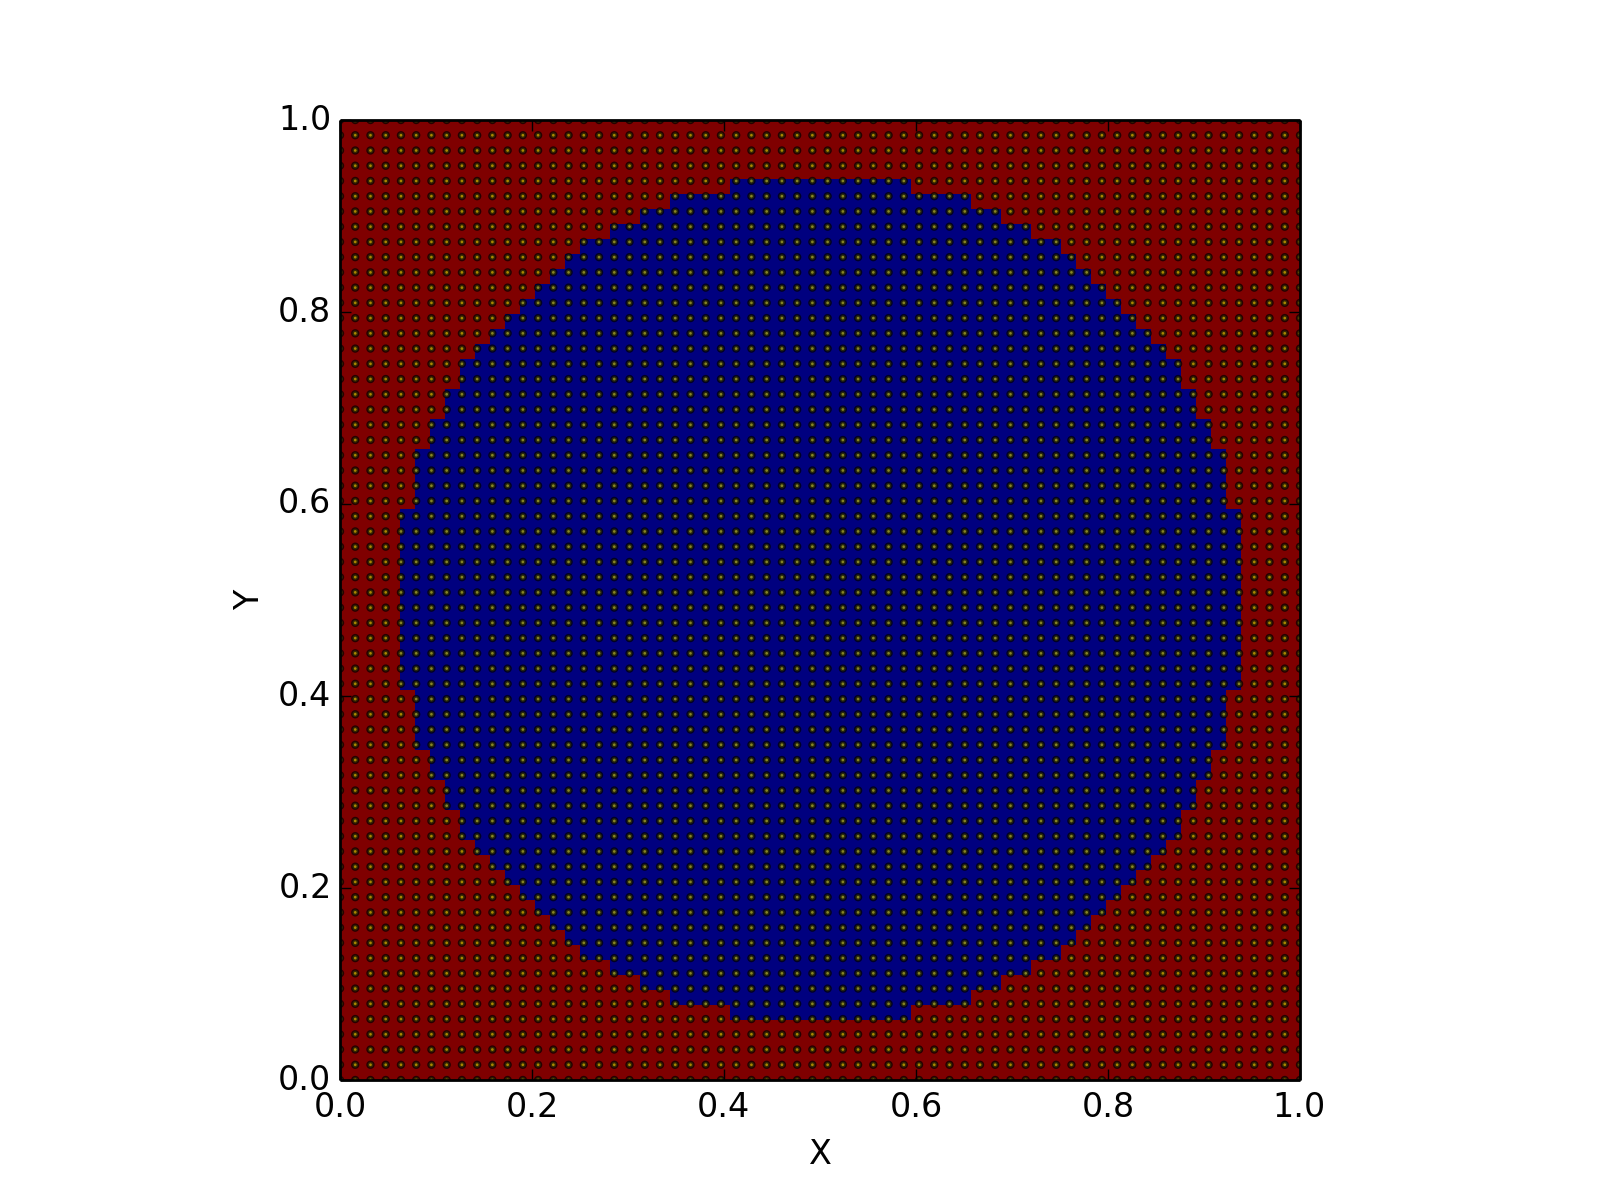
\includegraphics[width=0.5\textwidth]{gfx/immersed_boundary/mask.png}\label{fig:mask_vp}
        }}%
    \subfloat[Masking function $H(x,y,z=const.) = x^2 + y^2 < c$ for a cylinder. ]{{
      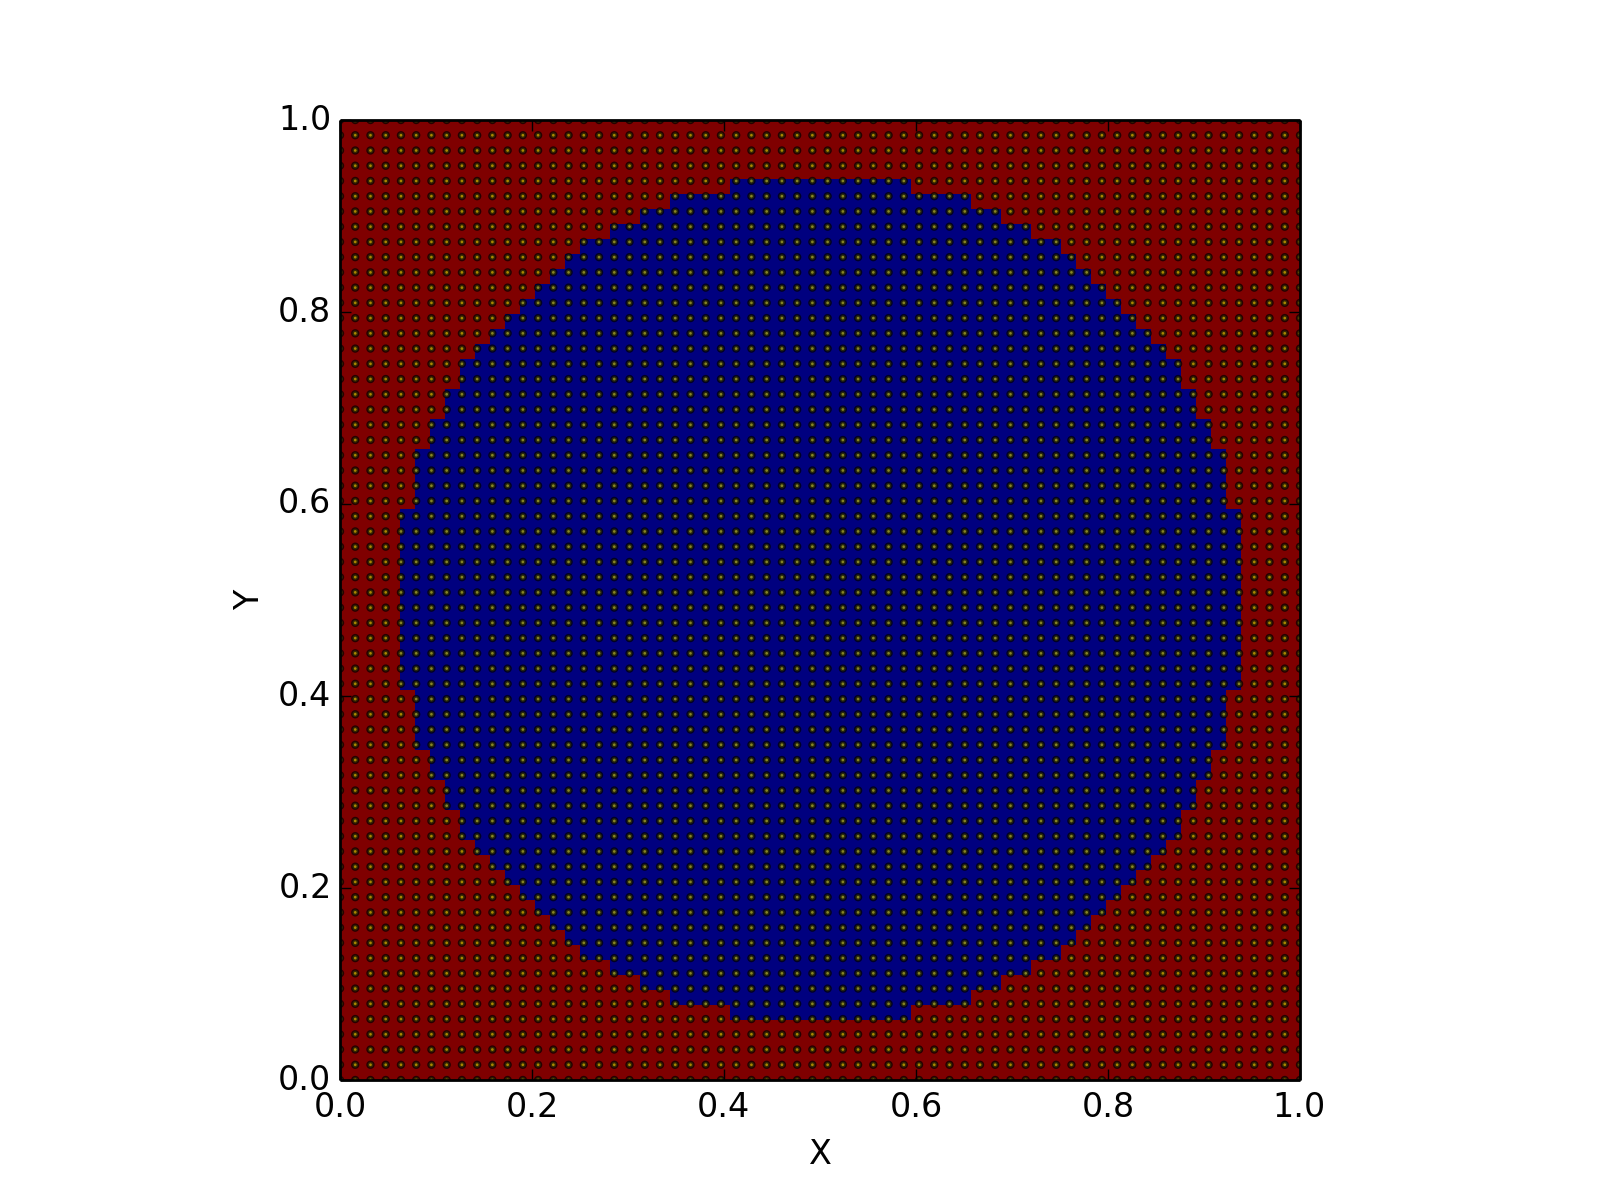
\includegraphics[width=0.5\textwidth]{gfx/immersed_boundary/mask.png}\label{fig:mask_vp}
     }}%
    \label{fig:example}%
\end{figure}

The idea behind the volume penalization method is to introduce an additional forcing term into the Navier-Stokes equation, which acts on
the grid points outside of the fluid domain to ensure the desired boundary conditions. The methods was sucessfully implemented and tested
on pseudo-spectral methods, see for example (CITE).
For the implementation it is necessary to define a masking function $H(x, y, z)$ which seperates the simulation domain into $\Omega_f$ and $\Omega_w$.
In case of the cylinder, we can use the surface equation (REF) and simply obtain.
\begin{align}
    \label{ibm:masking_function}
H(x, y, z) = \begin{cases}
                    0, &  \left(x - \frac{l_x}{2}\right)^2 + \left(y - \frac{l_y}{2}\right)^2 <r^2\\
                    1, & \text{else}
             \end{cases}
\end{align}
Now we can introduce an additional forcing term into the impulse equation,
\begin{align}
    \pdn[u]{t} + \vec{u} \cdot \vec{\nabla} \vec{u} &= -c^2 \nabla \rho + \frac{1}{Re} \Delta \vec{u} + \vec{F}_{ext}
     +\underbrace{ \frac{H(x, y, z)}{\nu}(\vec{v} - \vec{v_0})}_{\text{damping force}}
\end{align}

where $\vec{v}_0$ conforms the desired boundary condition, i.e. $\vec{v}_0 = 0 $ for no slip boundaries, and $\nu$ is a regulation parameter also denoted as damping rate of the forcing.
The additional term acts as an exponential damping force on a single gridpoint inside of $\Omega_w$, by the product with since it vanishes in $\Omega_f$ by the definition of $H(x,y,z)$.


Die Antwort des Kraftterms wird durch die Dämpfungrate $\nu$ reguliert. Je kleiner $\nu$ desto stärker ist die Dämpfungsrate, allerdings kann der Term
nicht beliebig klein gesetzt werden da die Stabilität für $\nu < dt$ nicht mehr gewährleistet ist [source].
Da für die Lösung der der Geschwindingskeitsfelder mit der Methode der künstliche Kompressibilität  bereits ein sehr kleiner Zeitschritt verwendet wird (s.Abb. X)
kann im Vergleich zu anderen Verfahren wie z.B. (pseudo-spektrale) eine relativ starke Dämpfungsrate verwendet werden.
-konvergenz nu gegen 0 MPI\\
- stiff probplem dt < dtpen = nu DIPLOM\\
- dary type law MPI\\
\newpage


\subsection{Direct Forcing}
Während die Volume Penalization Methode die Geschwindigkeit ausserhalb des Volumens nicht vollständig auf Null setzt,
 kann dies durch eine implizite Berechnung des Dämpfungsterm erreichtwerden. Es stellt sich heraus das dieser Ansatz equivalent
  zu der Direct Forcing Methode ist, die erstmals von [] verwendet und in [] beschrieben wird.
Betrachten wir zunächst den diskretisierten Zeitschritt
\begin{align}
    \frac{\vec{u}^{n+1} -\vec{u}^n}{\Delta t} = \mathscr{L} + \vec{f}\\
\end{align}
wobei $\mathscr{L}$ den diskretiesierten Operatoren der PDE entspricht.
Für einen Punkt auf dem Rand des Volumens soll nun die Randbedingung $\vec{u}^{n+1} = \vec{u}_0$ eingehalten werden.
Mit Formel () folgt
\begin{align}
    \frac{\vec{u}_0 -\vec{u}^n}{\Delta t} = \mathscr{L} + \vec{f} \Rightarrow \vec{f} = \frac{\vec{u}_0 -\vec{u}^n}{\Delta t\cdot \mathscr{L}}\\
\end{align}

Mit der Annahme dass der Rand mit dem numerischen Gitter übereinstimmt ist es nicht nötig den Kraftterm zur berechnen, stattdessen lässt sich der
Schritt vereinfachen in dem der Randwert nach  jedem Zeitschritt direkt auf die gewünschte Randbedingung gesetzt wird. Durch die
implizite Behandlung kommt es zu keiner weiter Stabilitätsbedingung.

\newpage

\subsection{Volume Fraction Interpolation}

The methods introduced up to here lack the ability of an exact impementation of the boundary conditions on $\Omega_f$.
Instead the surface $\partial \Omega_f$ is described by the nearest grid points in $\Omega_w$, resulting in an
stepwise approximation.
To overcome this problem a simple procedure is the use of an volume fraction interpolation scheme, introduced in [FADL].\\
The advantage of this method is the simple implementation into the volume penalization and direct forcing method.
Furthermore the overall computation time of the timestep stays constant, in  contrast to complex interpolation schemes.\\
Initially the interpolation beginns by determine all grid cells\footnote{definition cell} which are cut by the surface $\partial \Omega_f$.
For each of these boundary cells the total volume $V_w$ of the wall domain $\Omega_w$, inside each cell, is computed.
The force acting on the points inside the boundary cells is than weighted by a scaling factor, $\Phi = V_W/(\Delta x \Delta y \Delta z)$.
For the volume penalization method the scaling is simply multplied with the forcing term in eq. ().
Since the implementation of the direct forcing method is setting the velocity components directly to zero, it is necessary to
fall back to equation () and introduce a forcing term

\begin{align}
    \vec{f} = \Phi \frac{\vec{u}_0 -\vec{u}^n}{\Delta t\cdot \mathscr{L}}\\
\end{align}

\begin{figure}[!bp]
    \centering
    \subfloat[label 1]{{
      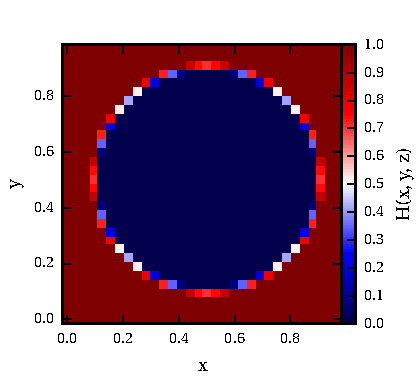
\includegraphics{gfx/immersed_boundary/methods/mask_volfrac.pdf}\label{fig:mask_volfrac}
        }}%
    \qquad
    \subfloat[label 2]{{
      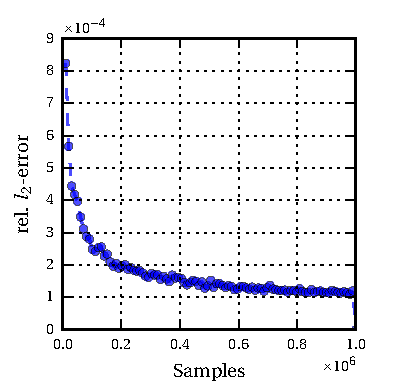
\includegraphics{gfx/immersed_boundary/methods/error_volfrac.pdf}\label{fig:error_volfrac}
        }}%
    \label{fig:example}%
\end{figure}

Since the operator $\mathscr{L}$ is computed during the first part of the time step. This forcing term can added during the completion of the runge kutta step.\footnote{see section}\\
For the implementation of an extended version of the masking array $H$ is used.
Like in the previous methods the masking array is precomputed and loaded at runtime. The algorithm is extended to compute the
volume fractions of the cells lying next to the surface $\partial\Omega_f$.
Since an exact computation is difficult to implement for abritary surfaces, the idea is to use a monte carlo integration method.
For each cell $N$ random samples are generated, then the volume fraction is simply given by the ratio of samples lying in- and outside ot the domain.
The implementation into a simulation class using the python API is explained in more detail in Appendix ().\\
An example for the computed masking array with $N=2e5$, is shown in figure (). The symmetric distribution of the boundarie values indicates
a good approximation, for a better evaluation a convergence study was performed were the number of samples $S$ was varied between 100 and $10^6$ points.
The $l_2$-error was determined by comparing the results to the computation with the highest number of samples.
The results are shown in figure ().\\
For the number of samples in the intervall below $S=2\dot10^5$, we can observe a fast decrease in the error to the order $2\dot10^{-4}$.
Above this intervall the overall decrease is of order $10^{-5}$ in the total error.
The global error of $2\dot10^-5$ is at least two orders below the error the interpolation methods introduce into the finite difference scheme, as we will see
in section (). Therefore we conlude that the volume fraction calculation should be accurate enough with $S=10^5$ samples.\\
%Finally we want to propose an enhancement to the volume fraction method. The idea behind the improvement can be stated as followed.
%Suppose we perform a simulation with a highly resolved numerical grid, in this case we can assume that the overall curvature of the boundary is negletable
%inside a single grid cell. This means that in the 2-dimensional case the boundary can be approximated by a straight line cutting the grid cell at a certain area.
%\begin{wrapfigure}{r}{0.5\textwidth}
%  \begin{center}
%    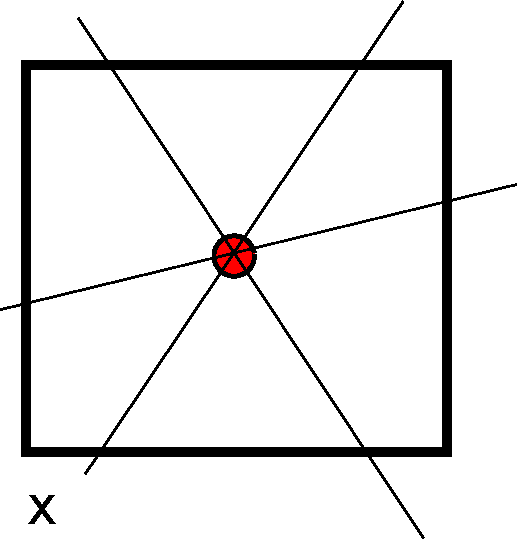
\includegraphics[width=0.3\textwidth]{gfx/immersed_boundary/methods/volfrac.pdf}
%  \end{center}
%  \caption{Example of surface cuts of grid cell}
%\end{wrapfigure}
%Now we examine the case where the calculated volume fraction is exactly $0.5$, this means that all possible surfaces have to cut the grid cell exactly in the middle.
%Therefore the grid point lies exacty on the surface and the overall velocity should be set to zero to fullfill the noslip condition.
%Our suggestion for the algorithm  is to multiply by a factor of two the volume fraction values and set all values above to the maximum value of one.

\clearpage
\subsection{Interpolation Method}

The last immersed boundary method introduced in this thesis is a bilinear interpolation method, which was first presented by \citep{Gilmanov2003}.
One difference to the previous methods is an exact representation of the immersed boundary, instead of a pixelated one.
A schematic representation of the interpolation procedure is shown in Fig. \ref{ibm:ip_method_algo}.

\begin{figure}[!bp]
      \centering
        \resizebox{0.8\textwidth}{!}{
       \import{gfx/immersed_boundary/methods///}{ip.pdf_tex}
      }
      \caption{Interpolation of the velocity of the point $b$. The point $c$ is a projection from the point $a$ into the direction of the normal $\vec{n}$,
       onto the plane defined by the grid points $\alpha$, $\beta$, $\gamma$ and $\delta$. The immersed boundary is given by the masking function H(x,y,z).
       For the bilinear interpolation the coefficient $c_1$ and $c_2$ are used.
      }
    \label{ibm:ip_method_algo}
\end{figure}

The interpolation method is applied to all grid points which posess a nearest neighbor outside of the fluid domain.
In this setup this is true for the point $b$, for which the velocity $\vec{v}$, shall be interpolated.
The idea of this method is to linear interpolate $b$ into the direction of the normal $\vec{n}$, of the immersed boundary.
The intersection of the interpolation direction with the boundary is given by the point $a$, with the distance $\Delta h =[ab]$.
The point $b$ is  projected into the direction of the normal $\vec{n}$, onto the plane defined by
the nearest grid points $\alpha$, $\beta$, $\gamma$ and $\delta$.
After the position calculation of the point $c$, the velocitiy $\vec{v}(c)$ is obtained by a bilinear interpolation
of the velocities at the points $\alpha$, $\beta$, $\gamma$ and $\delta$, given by (\citep{numrecipes})

\begin{align}
    \vec{v}(c) =  \frac{1}{\Delta x\Delta y} \left(\vec{v}(\beta)(\Delta x -  c_1)(\Delta y -  c_2) +
            \vec{v}(\gamma)(\Delta x -  c_1)(c_2) +
            \vec{v}(\alpha)(  c_1)(\Delta y -  c_2) +
            \vec{v}(\delta)( c_1)(c_2) \right)
\end{align}

where $(c_1, c_2)$ is the offset from $c$ to $\beta$, or in general the offset to the point of the plane, which is closest to $b$.

With the obtained velocity $v(c)$ and  the No-Slip boundarie condition $v(a) = 0$,
the interpolated velocity is given by
\begin{align}
    \vec{v}(b)  =  \vec{v}(c)\frac{\Delta c}{\Delta h}
\end{align}
where $\Delta c = [ac]$.

For a simplification of the interpolation procedure for different geometries, a preprocessing routine was implemented.
In order to interpolate a certain geometry three functions have to defined.
A masking function $H(x, y, z)$, a function which gives the distance to the boundary $d(x, y, z)$
and a function $\vec{g}(x, y, z)$ with determines the normal direction  of the boundary.
For the cylinder the masking function $H(x, y, z)$ is given by Eq. \ref{ibm:masking_function}.
The distance is

\begin{align}
    d(x, y, z) = \sqrt{\left(x - \frac{l_x}{2}\right)^2 + \left(y - \frac{l_y}{2}\right)^2  - r^2}
\end{align}

and the normal direction
\begin{align}
    \vec{g}(x, y, z) = \left(-\left(x - \frac{l_x}{2}\right),  - \left(y - \frac{l_y}{2}\right), 0\right)^T
\end{align}

A normalization of $\vec{g}(x, y, z)$ is performed in the algorithm,
however it is required that the normal  vectors point into the direction of the fluid domain.
Before the execution of a simulation the following steps are precomputed

\begin{enumerate}
    \item The closest point to $b$, in the example  $\beta$ is determined by the direction where $\vec{n}$ is the largest, in this example
          the $z$-direction with $n_0 := \max(\vec{n}) = n_z$.

    \item The points $\alpha$, $\gamma$, $\delta$ are determined by the remaining components ${n_y, n_z}$, which are used as directions to
            compute the offset from $\beta$.

    \item The offset $p00$, $p01$, $p10$, $p11$ of the points $\beta$, $\alpha$, $\gamma$, $\delta$ to the point $b$ are computed

    \item $\vec{n}$ is normalized by $\vec{n}^* = \frac{\vec{n}}{|n_0|}\cdot \Delta z$.
            \footnote{For $n_0=n_z$ this is $\Delta x$ and for $n_0=n_y$ it is $\Delta y$}

    \item The point $c$ is given by $c = a + \vec{n}^*$ and the coefficient $c_1$ and $c_2$ are computed and normalized to the values
           $c01 := \frac{c_1}{\Delta x}$ and $\c10 := \frac{c_1}{\Delta y}$.
    \item The ratio $W=\frac{\Delta c}{\Delta h} = \frac{d(x, y, z)}{d(x, y, z) + |\vec{n}| }$ is computed
\end{enumerate}

The values obtained from this precomputation are the offsets  $p00$, $p01$, $p10$, $p11$, the coefficients $c01$, $c10$ and
the ratio $W$. Each values is stored into an array of shape $N_x \cdot N_y \cdot N_z$, which is loaded during the simulation.
All values in the coefficient arrays which are not close to the immersed boundarie are set to zero.
During the interpolation procedure the ratio $W$ is checked and if larger than zero an interpolation for the grid point is computed.
An example of the interpolation procedure is given by

\begin{Verbatim} [fontsize=\footnotesize]
    if ((distance != 0 )){
      //load points of the plane (alpha, beta, gamma, delta)
      p00 = p00_d[global_Point] + global_Point;
      p01 = p01_d[global_Point] + global_Point;
      p10 = p10_d[global_Point] + global_Point;
      p11 = p11_d[global_Point] + global_Point;
      //load coefficients
      c01 = c01_d[global_Point];
      c10 = c10_d[global_Point];

      if (threadIdx.z == 1){
        //load velocities
        f00 = vx_d[p00]; f01 = vx_d[p01]; f10 = vx_d[p10]; f11 = vx_d[p11];
        //bilinear and linear interpolation
        f = W*(f00*(1 - c10)*(1 - c01) + f10*c10*(1 - c01)
                             + f01*c01*(1 - c10) + f11*c01*c10);
        //set the interpolated value
        vx_d[global_Point] = f;
      }
      if (threadIdx.z == 2){
        f00 = vy_d[p00]; f01 = vy_d[p01]; f10 = vy_d[p10]; f11 = vy_d[p11];
        f = W*(f00*(1 - c10)*(1 - c01) + f10*c10*(1 - c01)
                                + f01*c01*(1 - c10) + f11*c01*c10);
        vy_d[global_Point] = f;
      }
      if (threadIdx.z == 3){
        f00 = vz_d[p00]; f01 = vz_d[p01]; f10 = vz_d[p10]; f11 = vz_d[p11];
        f = W*(f00*(1 - c10)*(1 - c01) + f10*c10*(1 - c01)
                             + f01*c01*(1 - c10) + f11*c01*c10);
        vz_d[global_Point] = f;
      }
\end{Verbatim}

where \texttt{global\_Point} is the position of the interpolated point.
The performance of this implementation in comparsion to

\clearpage

